\chapter{Localizing and Mapping in Large-scale GPS-denied Scenarios}

\section{Introduction}

The localization system developed in this work is a Particle Filter Localization (PFL) algorithm that processes the vehicle's odometry to make predictions of the car movement considering an Ackerman kinematic model [15]. For the filter update, two different ways to compute the map-matching stage were implemented in order to reduce the computational cost of the localization process and to increase the accuracy of the vehicle pose estimates. The first distance is an improvement of the Likelihood Field Map-Matching. The second is the Cosine between the a-priori grid-map (off-line map) and the local grid-map, both represented as vector entities. The initialization of the PFL's particles uses external localization resources, such as low quality GPS and magnetometer's measurements.

\section{Large-Scale Environment Mapping System}
\label{sec:Mapping}

Our system design aims to solve large-scale mapping issues and to achieve a high mapping quality instead of focusing on exceptional computational performance. The architecture of the Large-Scale Environment Mapping System (LEMS) is illustrated in Figure \ref{Fig::FIGURE02}. In the first step, the Road-Map Localization System is run to determine the Global Car Path (GCP) simulating a GPS, besides the vehicle odometries information by Visual-LiDAR Odometer. 


\begin{figure}[ht]
    \centering
    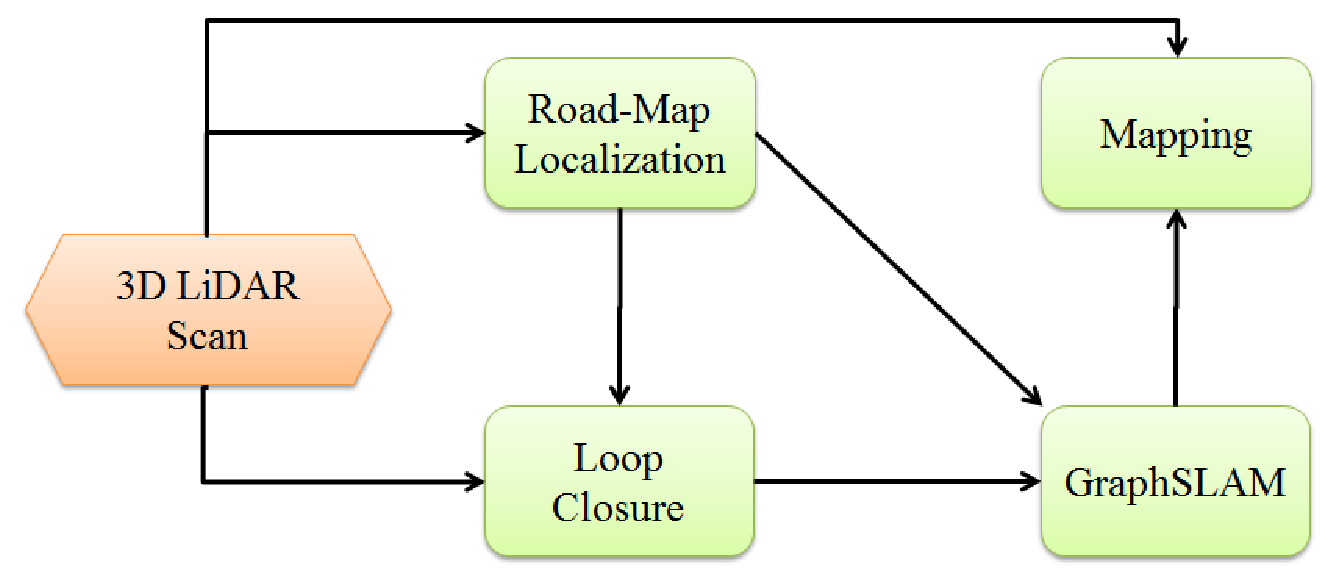
\includegraphics[width = 100 mm]{GraphSLAM.eps}
    \caption{Large-Scale Environment Mapping System (LEMS) Architecture. Firstly, a human drives IARA through the interest region and the sensor data are logged. Then, the Road-Map Localization system is executed to generate the Global Car Position and Visual-LiDAR Odometry. After that, the Loop Closure subsystem is used to detect revisited regions and to measure the displacement between the poses in the subsequent visits. Finally, the GraphSLAM subsystem is executed to estimate a feasible vehicle path and the Mapping subsystem is executed to build the environment grid map by projecting the velodyne point cloud from 3D to 2D, detecting obstacles, and placing them in the world using the GraphSLAM poses.}
    \label{Fig::FIGURE02}
\end{figure}

The Loop Closure subsystem receives as input the data from GCP and Velodyne point clouds, detects loop closure regions and estimates the displacement between the poses in the subsequent visits to the same region. The output of the loop closure subsystem, the data from Global car path and odometry are used to introduce restrictions to the GraphSLAM optimizer that is responsible for calculating the set of most likely poses given sensor data. Lastly, the mapping subsystem receives as input the Velodyne point clouds and the respective poses, calculated by the GraphSLAM, and outputs the environment occupancy grid map. It is important to note, however, that the proposed architecture can be easily extended to create any kind of grid map (e.g., re-emission grid maps, likelihood field grid maps, etc.).


\subsection{Loop Closure}

The loop closure subsystem has two objectives: firstly, to detect the poses of the robot when it revisits a region, and secondly, to measure the displacement of the poses in relation to the first visit caused by the dead-reckoning accumulated error.

To detect whether some region has already been visited, each GCP position data is compared with older GCP positions. If some old position has a smaller distance from the current GCP position than a pre-defined threshold (five meters, in this work) and the timestamp difference is bigger than a pre-defined threshold (in this work two minutes is used), a new loop closure is detected. In this case, both positions (the current one and the old one) are sent to the displacement measurement phase. If more than one position satisfies the loop closure condition, only the closest one is considered.

To estimate the displacement between two loop closure poses, we translate the Velodyne point clouds to the poses given by the GCP pose. Then, we register the point cloud of the second visit to the point cloud of the first visit using the GICP. This algorithm estimates the correction transformation that best fit a source point cloud to a target point cloud.

\subsection{GraphSLAM}

The GraphSLAM is a full-SLAM algorithm \cite{10thrun2006graph} in which the probabilistic variables are represented by graph vertices, and the sensor measurements are represented by graph edges. In this work, each vertex represents a robot pose (x-y and $\theta$) and edges correspond to sensor measurements and its uncertainties (represented as covariance matrices). Note that the GraphSLAM edges are the dead-reckoning, the loop closures and the GCP. Figure \ref{Fig::FIGURE03} illustrates an example of a graph.

\begin{figure}[ht]
    \centering
    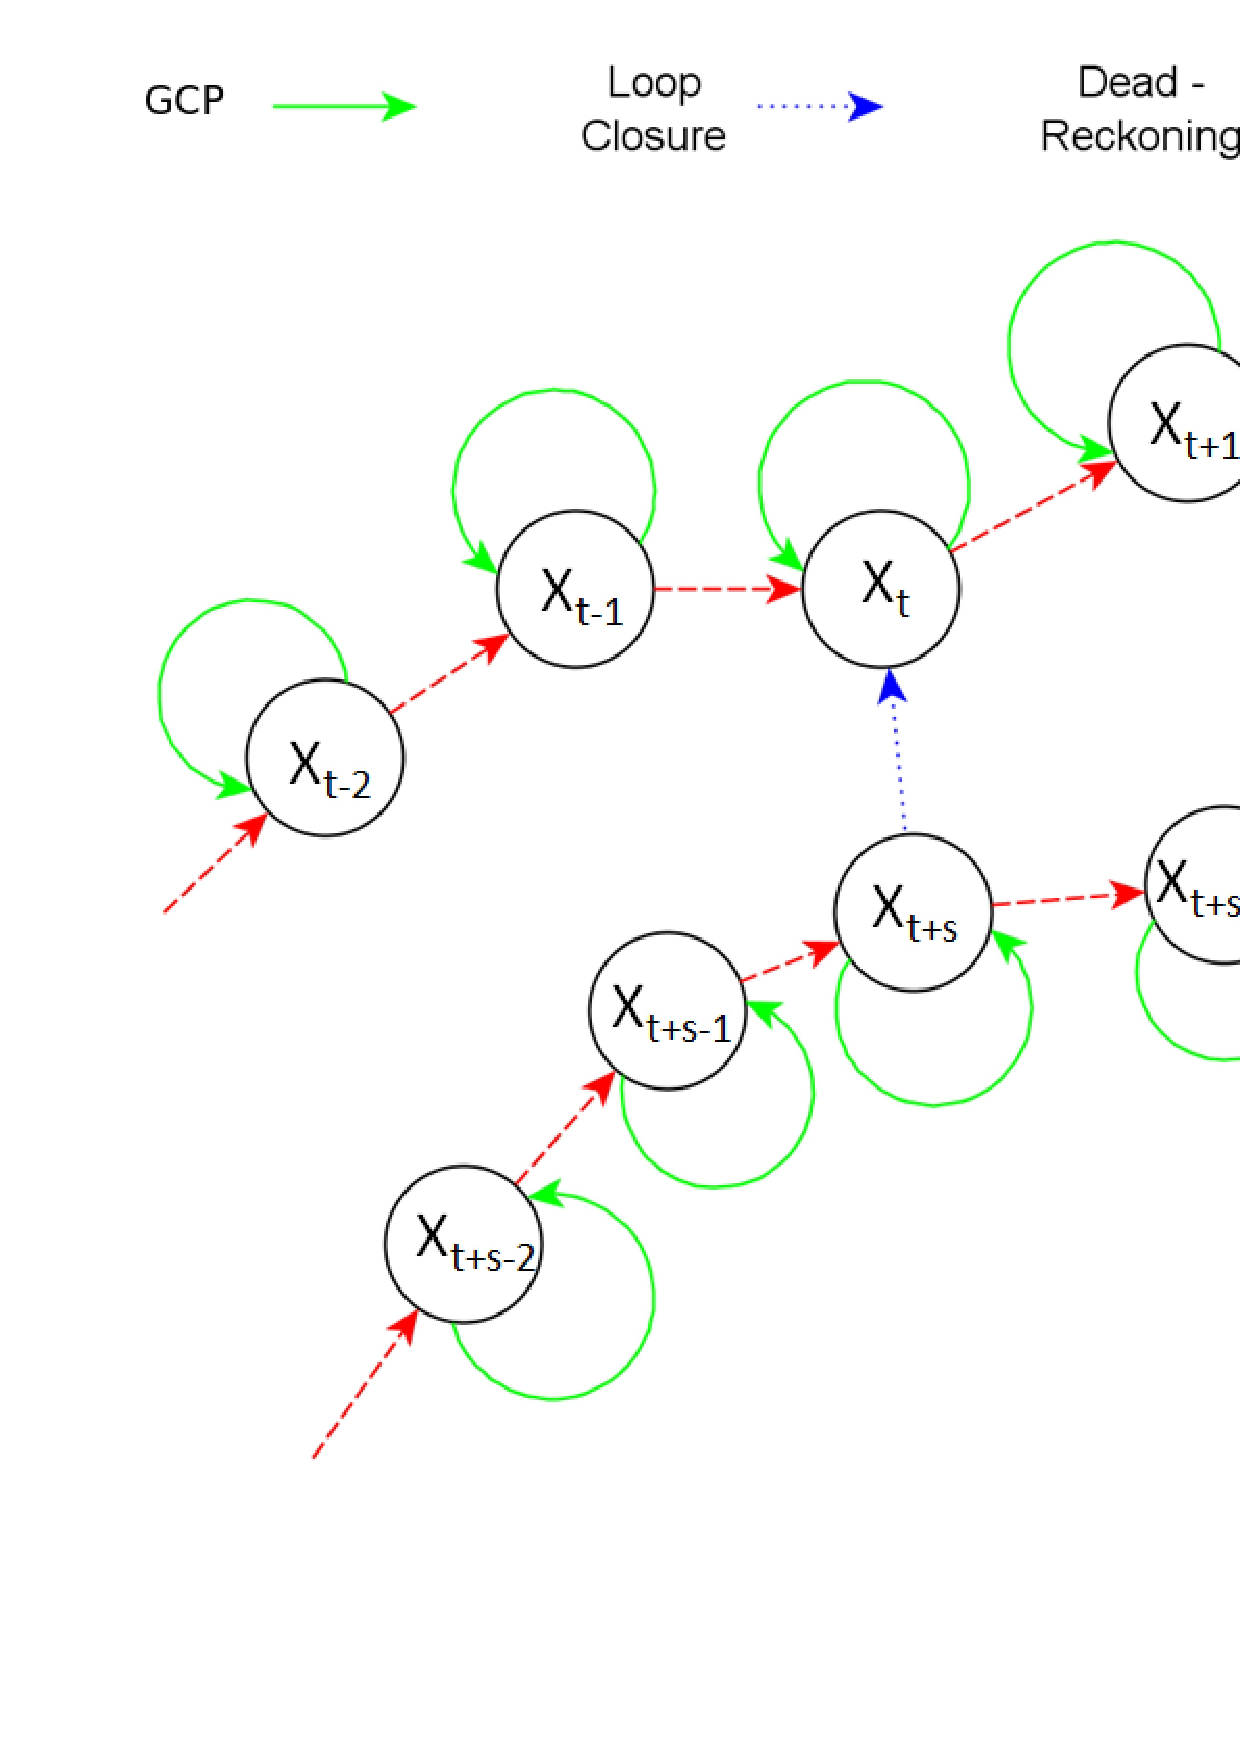
\includegraphics[width = 100 mm]{FIGURE03}
    \caption{Example of Graph Constructed by GraphSLAM. The black circles represent the poses, the red dashed edges represent the dead-reckoning displacements between two consecutive poses, the green filled unitary edges represent the GCP measurements, and the blue dotted edges represent the loop closures restrictions.}
    \label{Fig::FIGURE03}
\end{figure}

To estimate the most likely poses given the graph, several maximum-likelihood estimation techniques can be used. In special, when the sensor uncertainties are Gaussian, the maximum-likelihood estimation problem can be translated in a quadratic optimization problem solvable by gradient-based algorithms. The objective function of our GraphSLAM version is given by:
\begin{equation}
\label{Eq::GSLAMOBJ}
J=R_O+R_G+R_L
\end{equation}
where $R_O$ is the sum of odometry restrictions, $R_G$ is the sum of GCP restrictions, and $R_L$ is the sum of loop closure restrictions.

Because dead-reckoning and loop closure leads to Gaussian displacement restrictions and GCP lead to Gaussian global position restrictions, the log-likelihood objective function can be defined as:
\begin{equation}
\label{Eq::GSLAMlikelihoodOBJ}
\begin{array}{c}
J = \sum_{t}\left[ (X_t-(X_{t-1}+\delta_{t-1, t}))^TQ_t^{-1}(X_t-(X_{t-1}+\delta_{t-1, t}))\right]  \\
 + \sum_{t}\left[ (X_t-Y_t)^T R_t^{-1}(X_t-Y_t)\right]  \\
 + \sum_{X_A,X_B\in Loops}\left[ (X_B-(X_A+\delta_{X_A, X_B}))^TS_{X_A,X_B}^{-1}(X_B-(X_A+\delta_{X_A, X_B}))\right]
\end{array}
\end{equation}
where $X_t$ is a pose in time $t$,  $\delta_{t-1, t}$ is the estimated displacement between two consecutive poses $X_{t-1}$ and $X_t$ from dead-reckoning, $Y_t$ is a GCP measurement in time $t$, $\delta_{X_A, X_B}$ is a displacement from the pose $X_A$ to the pose $X_B$ (estimated by GICP) and $Q_t^{-1}$, $R_t^{-1}$ e $S_{X_A,X_B}^{-1}$ are the inverse covariance matrices from dead-reckoning, GCP and loop closure, respectively. During the optimization, the poses ($X_t$,$X_{t-1}$, $X_A$ and $X_B$) are changed and the sensors observations ($\delta_{t-1, t}$, $Y_t$ and $\delta_{X_A, X_B}$) and covariance matrices ($Q_t$, $R_t$ and $S_{X_A,X_B}$) stay fixed.


The mapping subsystem receives as input the Velodyne point clouds and its respective poses calculated by the GraphSLAM and outputs grid maps of the visited environment. The mapping used here is the same described in Section \ref{sec::ch2-mapping}. However, one important concern regarding mapping large-scale environments is the amount of memory used to store the map structure. A memory overflow can happen if the whole map is held in memory and the environment is sufficiently big. Taking this into account, we implemented a sub-map technique in which the mapped environment was divided in blocks of $50\times50$ meters, all of them with 0.2 meters of grid resolution (62,500 cells for each block). To reduce the memory consumption, the sub-map manager loads the blocks from the Hard Disk (HD) to the main memory in groups of nine blocks. It groups the small blocks to create a larger one with $150\times150$ meters. In addition, the sub-map manager is responsible for monitoring if the robot is in the central sub-map. When the robot crosses the central block boundaries, the sub-map manager loads new sub-maps to main memory and saves in HD and frees from memory the sub-maps that are not required anymore.

Figure \ref{Fig::FIGURE05} illustrates the procedure to switch sub-maps. The vehicle is initially located in the sub-map 4 (central block), and it begins to move in the direction of the sub-map 1 (Figure \ref{Fig::FIGURE05A}). Once the robot crosses the central sub-map boundary, three new sub-maps are loaded (9, 10 and 11) and incorporated into the sub-map held in memory (Figure \ref{Fig::FIGURE05B}). After that, the sub-map 1 becomes the new central sub-map and the sub-maps 6, 7 and 8 are saved in the Hard-Disk (HD) and freed from the main memory (Figure \ref{Fig::FIGURE05C}). Finally, the sub-maps are renamed as showed in Figure \ref{Fig::FIGURE05A}.

\begin{figure}[t]
\centering
\subfloat[]{
\begin{tabular}{|c|c|c|}
\hline
0 & 1 & 2 \\ \hline
3 & 4 & 5 \\ \hline
6 & 7 & 8 \\ \hline
\end{tabular}
\textbf{\label{Fig::FIGURE05A}}
}
\subfloat[]{
\begin{tabular}{|c|c|c|}
\hline
9 & 10 & 11 \\ \hline
0 & 1 & 2 \\ \hline
3 & 4 & 5 \\ \hline
6 & 7 & 8 \\ \hline
\end{tabular}
\label{Fig::FIGURE05B}
}
\subfloat[]{
\begin{tabular}{|c|c|c|}
\hline
9 & 10 & 11 \\ \hline
0 & 1 & 2 \\ \hline
3 & 4 & 5 \\ \hline
\end{tabular}
\label{Fig::FIGURE05C}
}
\caption{Illustration of the sub-map management technique. In all figures, each cell represents a $50\times50$ meter sub-map. The set of cells creates a $150\times150$ meters map that is used by the robot to localize itself and to navigate on the environment. At each instant, the robot "lives" only in the central sub-map. Whenever it crosses the boundary of the central sub-map, new sub-maps are loaded from HD to compose the new map in memory. Thereafter, the unnecessary sub-maps are saved on the disk and cleaned from the main memory. (a) $150\times150$ meters map that is kept on the main memory of the computer. (b) transition when the robot crosses the boundary of the central map and some of new sub-maps are loaded. (c) saving and freeing of the sub-maps that are no longer necessary.}
\label{Fig::FIGURE05}
\end{figure}

\section{Localization System}

The localization system developed in this work is a Particle Filter Localization (PFL) algorithm that processes the Visual-LiDAR Odometry to make predictions of the car movement. For the filter update, two different ways to compute the map-matching stage were implemented and evaluated in order to reduce the computational cost of the localization process and to increase the accuracy of the vehicle pose estimates. The first distance is an improvement of the Likelihood Field Map-Matching. The second is the Cosine between the a-priori grid-map (off-line map) and the local grid-map, both represented as vector entities.

\subsection {Online Map Construction}
Differently from the offline grid map ($m$), the local grid-map ($m_{local_{t}}$) is constructed on-the-fly by the techniques introduced in Section  \ref{sec::ch2-mapping}. It is an occupancy grid-map based on just one Velodyne twist scan at the time $t$, as shown in Figure \ref{Fig::OCU-ONE-SHOt}. As the map-matching distances do only consider the grid cells that represent obstacles in the local map, the set of selected grid cells is consequently very sparse. The local map is compacted by using the Compressed Row Storage (CRS) techniques \cite{bai2000templates}. 

The CRS stores the known cell values of the local map using three vectors, one vector for cell values, other for cell columns index, and the last one for the index in both other vectors (values and columns), where each line of the local map starts. In many cases this policy dramatically reduces (e.g. to just 3\%) the number of map queries for each particle. We consider as a map queries individuals access (reading) to the grid-cells during the process of the particle weight estimation. Figure \ref{Fig::VELODYNE-ONE-SHOT-MAP} shows the comparison between the number of point in one Velodyne twist scan (Figure \ref{Fig::POINT-CLOUD}) against the local map (Figure \ref{Fig::OCU-ONE-SHOt}). Consequently, the processing cost required in the map-matching stage is remarkably decreased. This stage is the most expensive operation in the process of localization using maps.

\begin{figure}[t]
\centering
    \subfloat[]{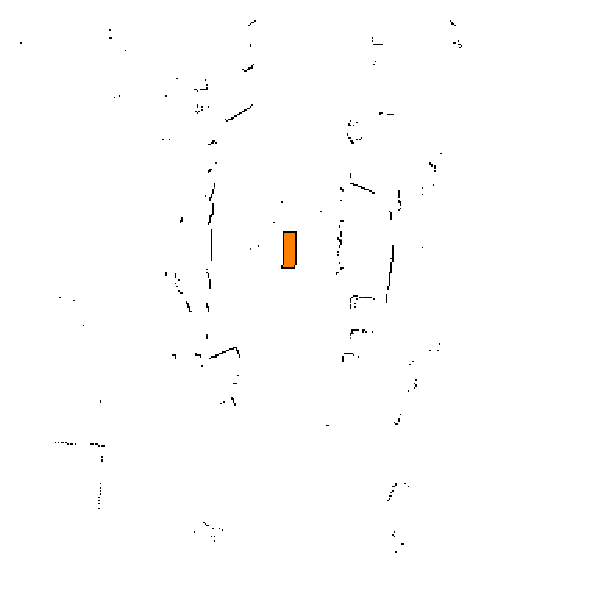
\includegraphics[width=50mm]{Occupancy-oneshot.eps}
    \label{Fig::OCU-ONE-SHOt}}
    \subfloat[]{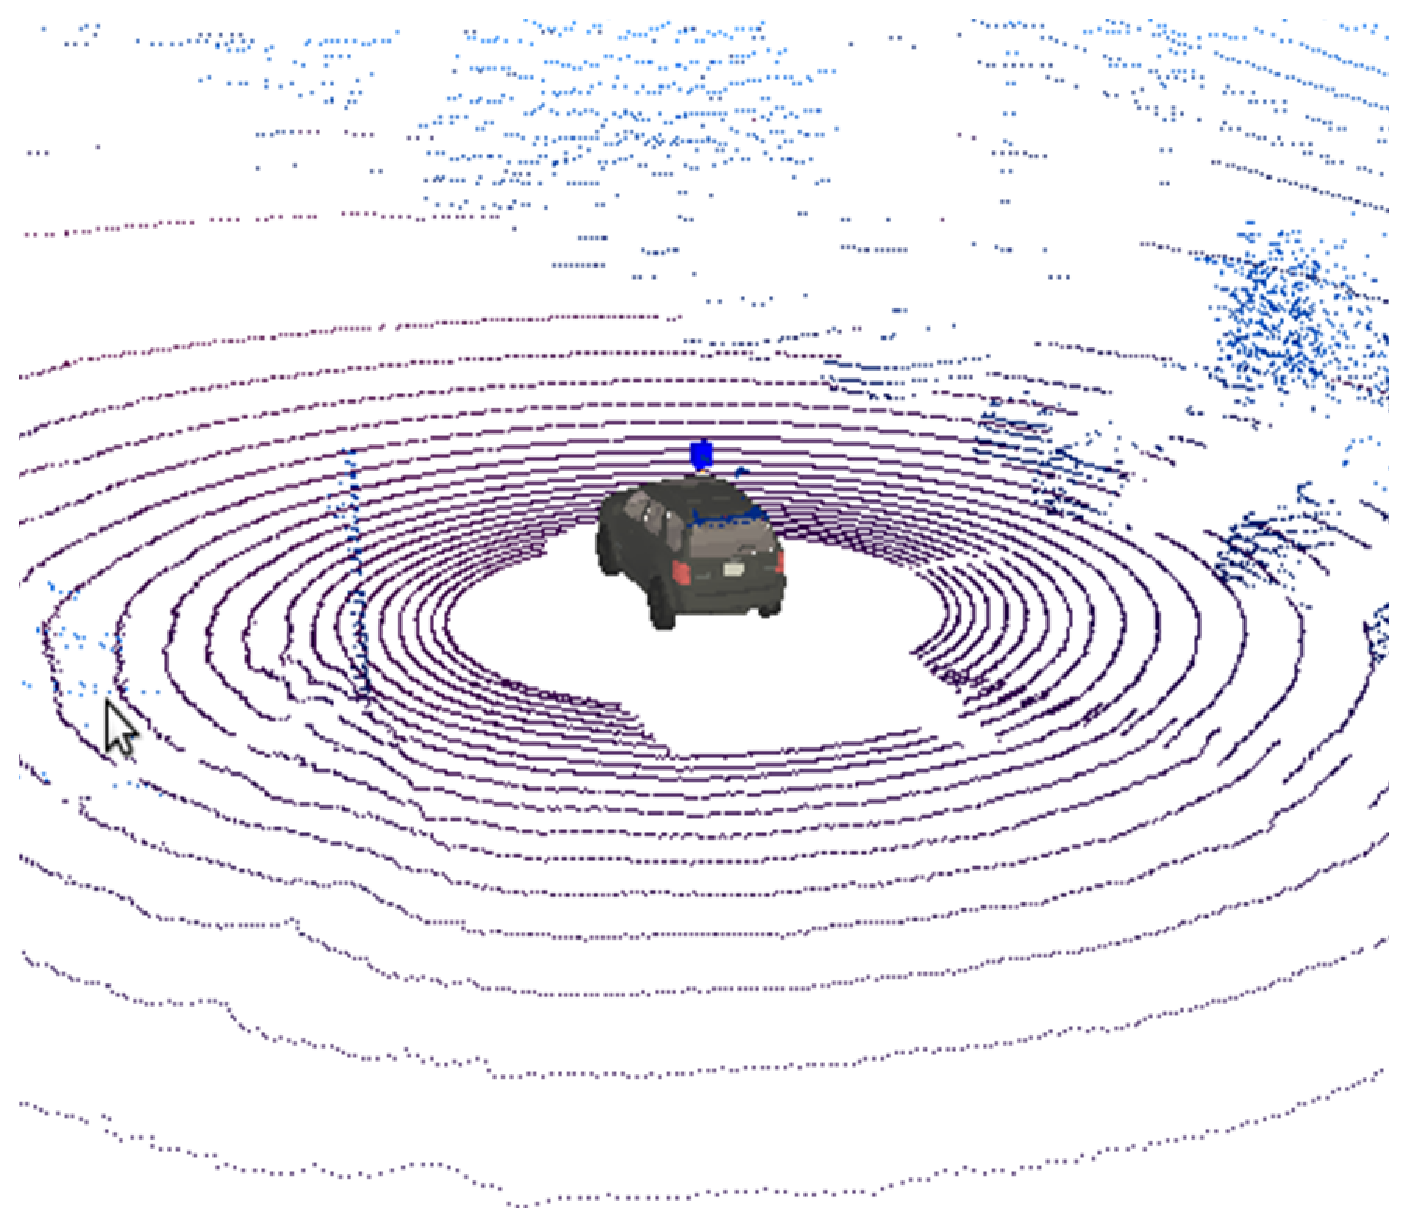
\includegraphics[width=60mm]{point-cloud.eps}
    \label{Fig::POINT-CLOUD}}
\caption{Local grid map based on measurements provided by a Velodyne 3D LiDAR sensor and projected to 2D (left). The black cells represent the obstacle identified in a Velodyne 3D imagery. The image illustrates part of a Velodyne point cloud in one spin (right). After mapping, the number of points that will be used to perform the map-matching was reduced severely.}
\label{Fig::VELODYNE-ONE-SHOT-MAP}
\end{figure}

\subsection{Particle Filter Localization}

The PFL is a probabilistic localization approach, which follows the recursive nonparametric Bayesian Filter, also known as Monte Carlo Localization \cite{26thrun2005probabilistic}. PFL represents the probability of the 3DoF pose $X=[x,y,\theta]$ (the position $x$ and $y$,and the orientation $\theta$) as a finite set of random particles. The set of particles is usually initialized by an uniform distribution over the workspace. Then, the filter runs iteratively, performing predictions about the robot movement and updates based on the measurements of the environment. For instance, after the initialization, the particles are sampled following the robot kinematic model using the odometry of the robot. This is usually called as prediction phase. When an exteroceptive measurement is available, an update step can be performed. In the update step, the generated local map is compared with the expected local map of each particle (based on the global offline map) in order to estimate the particles' weights. This phase is usually denominated the importance factor. Finally, the particles are drawn to select the most likely particles to compose the robot pose.

Generally, the PFL localizes the robot globally distributing the particles uniformly along the grid map $m$. Since the robot is running in outdoor places, in this work, the first position is selected manually as initial guess for the particles localization. Finally, the particles are sampled following a Gaussian distribution centered in the pose indicated and the covariance proportional (here, we are using 2 meters).
 
After its initialization step, the PFL runs iteratively in order to localize the vehicle using the provided a-priori map $m$. At each time step $t$, it predicts the vehicle motion, computes the particles weights and re-samples them. To estimate the vehicle motion from $t-1$ to $t$, the PFL uses the vehicle odometry data $u_t=\left\langle v_t,\omega_t\right\rangle $ ($v_t$ and $\omega_t$ are, respectively, the vehicle longitudinal and angular velocities) to generate a hypothetical vehicle motion. The estimation follows an Ackerman kinematic model that  moves a particle $k$ from the state $x_{t-1}^k$  to $x_t^k$ by adding Gaussian noise \cite{54sotelo2003lateral}. This phase involves sampling from the state transition distribution $p(x_t^k |u_t,x_{t-1}^k,m)$. The weight $w_t^k$ is computed for each particle $k$ by applying the map-matching distance between $m_{local_{t}}$ and m given $x_t^k$. The local map $m_{local_{t}}$  is aligned to grid map m given the pose of the robot in $m_{local_{t}}$ (central position) and $x_t^k$. At the end of each update step of the PFL algorithm, the particles are re-sampled to emphasize the most likely particles. The final estimation provided by the PFL to other client processes of the autonomous vehicle (such as the position controller) is the average of the values of the current particles population. 

\subsection{Log-Likelihood Map-Matching}

The high frequency localization proposed in this work computes the map-matching by summing the log of the likelihood in the Likelihood Field (LF) grid-map, specifically focusing on the grid cells that have a high probability of being an obstacle, in the local occupancy grid-map $m_{local_{t}}$. Eq.\ref{Eq::ch3-1} expresses the Log-Likelihood field distance estimation.
\begin{equation}
\label{Eq::ch3-1}
g(m_{local_{t}},x_t,m_{LF}) = \sum_{\forall(i,j)\in \Omega_t} \log(h(i,j,x_t,m_{LF}))
\end{equation}
where the subset $\Omega_t=\left\lbrace (i.j) \colon m_{local_{t}} (i,j)>0.5\right\rbrace $, i.e. cells which represent an obstacle. $m_{LF}$  is the Likelihood Field grid-map. $h(i,j,x_t,m_{LF})$  is a function that returns the value of a cell in the global grid map hit by a cell of the local map that was aligned (rotated and translated) given the hypothesis $x_t$. As a consequence of this policy, the number of map queries is remarkably reduced, making the full estimation process feasible to be performed in real-time. The weights for all the particles are evaluated based on the map matching instances, calculated for each of the particles. The particle weight $w_t^k$ for each particle $k$ is defined as follows:
\begin{equation}
\label{Eq::ch3-3}
w_t^k = \frac{\exp(g(m_{local_{t}},x_t^k,m_{LF}))}{\exp(\max_{i}(g(m_{local_{t}},x_t^i,m_{LF})))}
\end{equation}

\subsection{Cosine Map-Matching}

As an alternative to Log-Likelihood distance, we present the cosine distance to compute the map-matching. The Cosine between high dimension vectors has been used in Information Retrieval in order to measure the distance between two documents represented as vectors \cite{23baeza1999modern}. Due to its characteristics, the problem of map-matching is able to be treated in a similar way.

The Cosine distance evaluates the angular distance between two vectors in the $\Re^n$ space. In our approach, $n$ is the number of grid cells having $m_{local_{t}}(i,j)>0.5$. This measure evaluates the angular distance between know cells in $m_{local_{t}}$ and the corresponding cells in $m$. The Cosine distance is defined as follows:
\begin{equation}
\label{Eq::ch3-4}
cos(m_{local_{t}},x_t,m) = \frac{\sum_{\forall(i,j)\in \Omega_t} m_{local_{t}}(i,j) \cdotp h(i,j,x_t,m)}{\sqrt{\sum_{\forall(i,j)\in \Omega_t}m_{local_{t}}(i,j)^{2}}\sqrt{\sum_{\forall(i,j)\in \Omega_t}h(i,j,x_t,m)^{2}}}
\end{equation}
The Cosine distance varies between -1 and 1, where the lowest value represents the maximum dissimilarity and the highest one the maximum similarity. The negative values happen when most of the $m_{local_{t}}$ cells are aligned with unknown cells in $m$. This situation usually happens when a particle is placed in regions labeled to be unknown, or is placed close of them. To avoid such cases, the cosine is summed with one, $g(m_{local_{t}},x_t,m)=1+\cos(m_{local_{t}},x_t,m)$, and as a result the function output changes to $[0, 2]$. To compute the particles' weights, the function $g(\cdotp)$ is normalized. Then, the definition of the particles' weight is expressed according to the following expression:
\begin{equation}
\label{Eq::ch3-5}
w_t^k = \frac{g(m_{local_{t}},x_t^k,m) - \min_{i}(g(m_{local_{t}},x_t^i,m))}{\max_{i}(g(m_{local_{t}},x_t^i,m)) - \min_{i}(g(m_{local_{t}},x_t^i,m))}
\end{equation}
